\section{Test Case: Built-in Atmosphere Upwelling}
%=================================================

\subsection{Double precision linux results}
%------------------------------------------
The double precision results for the linux/gfortran system for the built-in atmosphere test case are shown in figure \ref{fig:run_example_built_in_atm_upwelling-dbl_gfortran}. Residuals for LBLRTM runs using the local and LNFL \texttt{TAPE3} spectroscopic input files are shown. Results using the AER \texttt{TAPE3} file were identical to the LNFL results.

\begin{figure}[htp]
  \centering
  \qquad\sffamily\textbf{Verification Example: Built-in Atmosphere Upwelling}\\
  \qquad\sffamily\textbf{Red Hat linux platform; gfortran; double precision}\\
  \qquad\textsf{LBLRTM v11.3 brightness temperature difference for \textbf{Local} \texttt{TAPE3} run}\\
  \includegraphics[bb=82 490 534 648,clip,scale=1.0]{graphics/run_example_built_in_atm_upwelling/gfortran/dbl.eps}
  \qquad\textsf{LBLRTM v11.3 brightness temperature difference for \textbf{LNFL} \texttt{TAPE3} run}\\
  \includegraphics[bb=82 313 534 472,clip,scale=1.0]{graphics/run_example_built_in_atm_upwelling/gfortran/dbl.eps}
  \caption{Built-in Atmosphere Test: Comparison of the AER-supplied \texttt{TAPE27\_ex} output to the locally generated \texttt{TAPE27} output for the \textsl{double precision} version of LBLRTM v11.3 running on a Red Hat linux system using the gfortran compiler. \mbox{\textbf{(a)} Using} the little-endian \texttt{TAPE3} spectroscopic datafile generated from the local input shown in figure \ref{fig:local_tape3_tape5}. \mbox{\textbf{(b)} Using} the little-endian \texttt{TAPE3} spectroscopic datafile generated from the LNFL v2.5 distribution input shown in figure \ref{fig:lnfl_ex_tape3_tape5}. This result is identical to the same using the \textbf{AER} little-endian \texttt{TAPE3} spectroscopic datafile.}
  \label{fig:run_example_built_in_atm_upwelling-dbl_gfortran}
\end{figure}

The anomaly seen in the optimised linux/gfortran results (see appendix \ref{app:busted_gfortran_compiler_results}) was the main reason an additional compiler, the PGI one, was used. The double precision results for the linux/PGI system are effectively identical to the gfortran results shown in figure \ref{fig:run_example_built_in_atm_upwelling-dbl_gfortran}.

The main residuals in figure \ref{fig:run_example_built_in_atm_upwelling-dbl_gfortran}(a) are due to the differences in how the  \texttt{TAPE3} files were generated; that is, fewer molecular species. A magnification of these individual line differences for the locally generated TAPE3 case is shown in figure \ref{fig:run_example_built_in_atm_upwelling-dbl_gfortran_1035.8-1035.9}. The character of the differences suggest a line width difference. This type of difference could be explained by to a differnt number of absorption lines (due to the different number of included absorbers in the \texttt{TAPE3} files) being included in a line summation over a particular range of frequencies. That, however, is a speculative hypothesis and, since using similarly generated \texttt{TAPE3} data makes those differences go away, not worthy of further investigation here.

\begin{figure}[htp]
  \centering
  \qquad\sffamily\textbf{Verification Example: Built-in Atmosphere Upwelling}\\
  \qquad\sffamily\textbf{Red Hat linux platform; gfortran; double precision}\\
  \qquad\textsf{LBLRTM v11.3 brightness temperature difference for \textbf{Local} \texttt{TAPE3} run}\\
  \includegraphics[bb=82 490 534 648,clip,scale=1.0]{graphics/run_example_built_in_atm_upwelling/gfortran/dbl_1035.8-1035.9.eps}
  \caption{Built-in Atmosphere Test: A magnification of the 1035.8-1035.9\invcm{} spectral region from figure \ref{fig:run_example_built_in_atm_upwelling-dbl_gfortran}(a) showing the typical residuals seen for the individual ``lines'' when \texttt{TAPE3} inputs files containing different numbers of absorbers are used. The PGI compiler also produced the same result.}
  \label{fig:run_example_built_in_atm_upwelling-dbl_gfortran_1035.8-1035.9}
\end{figure}

A feature of figure \ref{fig:run_example_built_in_atm_upwelling-dbl_gfortran}(b) is not visible at the y-axis scaling shown; a magnification of figure \ref{fig:run_example_built_in_atm_upwelling-dbl_gfortran}(b) is shown in figure \ref{fig:run_example_built_in_atm_upwelling-dbl_gfortran_noyshare}. The periodicity of the residuals is quite evident -- as is the residual line structure seen superimposed on the periodic differences -- although it must be pointed out that the magnitudes of the residuals are very small.

\begin{figure}[htp]
  \centering
  \qquad\sffamily\textbf{Verification Example: Built-in Atmosphere Upwelling}\\
  \qquad\sffamily\textbf{Red Hat linux platform; gfortran; double precision}\\
  \qquad\textsf{LBLRTM v11.3 brightness temperature difference for \textbf{LNFL} \texttt{TAPE3} run}
  \includegraphics[bb=75 313 534 472,clip,scale=1.0]{graphics/run_example_built_in_atm_upwelling/gfortran/dbl_noyshare.eps}
  \caption{Built-in Atmosphere Test: A magnification of figure \ref{fig:run_example_built_in_atm_upwelling-dbl_gfortran}(b) showing the periodic residuals. This result is identical to the same using the \textbf{AER} little-endian \texttt{TAPE3} spectroscopic datafile. The PGI compiler also produced the same result.}
  \label{fig:run_example_built_in_atm_upwelling-dbl_gfortran_noyshare}
\end{figure}


\subsection{Double precision AIX results}
%----------------------------------------
The double precision results for the AIX system for the built-in atmosphere test case are shown in figure \ref{fig:run_example_built_in_atm_upwelling-dbl_ibm}.

\begin{figure}[htp]
  \centering
  \qquad\sffamily\textbf{Verification Example: Built-in Atmosphere Upwelling}\\
  \qquad\sffamily\textbf{IBM AIX platform; double precision}\\
  \qquad\textsf{LBLRTM v11.3 brightness temperature difference for \textbf{Local} \texttt{TAPE3} run}\\
  \includegraphics[bb=82 490 534 648,clip,scale=1.0]{graphics/run_example_built_in_atm_upwelling/ibm/dbl.eps}
  \qquad\textsf{LBLRTM v11.3 brightness temperature difference for \textbf{LNFL} \texttt{TAPE3} run}\\
  \includegraphics[bb=82 313 534 472,clip,scale=1.0]{graphics/run_example_built_in_atm_upwelling/ibm/dbl.eps}
  \caption{Built-in Atmosphere Test: Comparison of the AER-supplied \texttt{TAPE27\_ex} output to the locally generated \texttt{TAPE27} output for the \textsl{double precision} version of LBLRTM v11.3 running on an IBM AIX system. \mbox{\textbf{(a)} Using} the big-endian \texttt{TAPE3} spectroscopic datafile generated from the local input shown in figure \ref{fig:local_tape3_tape5}. \mbox{\textbf{(b)} Using} the big-endian \texttt{TAPE3} spectroscopic datafile generated from the LNFL v2.5 distribution input shown in figure \ref{fig:lnfl_ex_tape3_tape5}. This result is identical to the same using the \textbf{AER} big-endian \texttt{TAPE3} spectroscopic datafile.}
  \label{fig:run_example_built_in_atm_upwelling-dbl_ibm}
\end{figure}

Similar magnifications of figure \ref{fig:run_example_built_in_atm_upwelling-dbl_ibm} as seen in figures \ref{fig:run_example_built_in_atm_upwelling-dbl_gfortran_1035.8-1035.9} and \ref{fig:run_example_built_in_atm_upwelling-dbl_gfortran_noyshare} show the IBM system produces the same residuals as the linux system.


\subsection{Single precision results}
%------------------------------------
\label{sec:built_in_sgl}
The single precision results for both the linux and AIX systems for the built-in atmosphere test case are shown in figures \ref{fig:run_example_built_in_atm_upwelling-sgl_gfortran} and \ref{fig:run_example_built_in_atm_upwelling-sgl_ibm} respectively. The two sets of results are effectively identical.

The size of the residuals are, however, slightly disconcerting. These residuals are determined from comparison between the AER-supplied double precision \texttt{TAPE27\_ex} result and the locally generated \texttt{TAPE27} result using a single precision build of LBLRTM v11.3.

\begin{figure}[htp]
  \centering
  \qquad\sffamily\textbf{Verification Example: Built-in Atmosphere Upwelling}\\
  \qquad\sffamily\textbf{Red Hat linux platform; gfortran; single precision}\\
  \qquad\textsf{LBLRTM v11.3 brightness temperature difference for \textbf{LNFL} \texttt{TAPE3} run}\\
  \includegraphics[bb=82 313 534 472,clip,scale=1.0]{graphics/run_example_built_in_atm_upwelling/gfortran/sgl.eps}
  \caption{Built-in Atmosphere Test: Comparison of the AER-supplied \texttt{TAPE27\_ex} output to the locally generated \texttt{TAPE27} output for the \textsl{single precision} version of LBLRTM v11.3 running on a Red Hat linux system using the gfortran compiler. The little-endian \texttt{TAPE3} spectroscopic datafile generated from the LNFL v2.5 distribution input shown in figure \ref{fig:lnfl_ex_tape3_tape5} was used. This result is the same as those produced using either the \textbf{Local} or \textbf{AER} little-endian \texttt{TAPE3} spectroscopic datafile.}
  \label{fig:run_example_built_in_atm_upwelling-sgl_gfortran}
\end{figure}

\begin{figure}[htp]
  \centering
  \qquad\sffamily\textbf{Verification Example: Built-in Atmosphere Upwelling}\\
  \qquad\sffamily\textbf{IBM AIX platform; single precision}\\
  \qquad\textsf{LBLRTM v11.3 brightness temperature difference for \textbf{LNFL} \texttt{TAPE3} run}\\
  \includegraphics[bb=82 313 534 472,clip,scale=1.0]{graphics/run_example_built_in_atm_upwelling/ibm/sgl.eps}
  \caption{Built-in Atmosphere Test: Comparison of the AER-supplied \texttt{TAPE27\_ex} output to the locally generated \texttt{TAPE27} output for the \textsl{single precision} version of LBLRTM v11.3 running on an IBM AIX system. The big-endian \texttt{TAPE3} spectroscopic datafile generated from the LNFL v2.5 distribution input shown in figure \ref{fig:lnfl_ex_tape3_tape5} was used.This result is the same as those produced using either the \textbf{Local} or \textbf{AER} big-endian \texttt{TAPE3} spectroscopic datafile.}
  \label{fig:run_example_built_in_atm_upwelling-sgl_ibm}
\end{figure}

So, what is the cause of the relatively large residuals when comparing the single precision calculations? Magnification of any of the panels of figures \ref{fig:run_example_built_in_atm_upwelling-sgl_gfortran} or \ref{fig:run_example_built_in_atm_upwelling-sgl_ibm}, as shown in figure \ref{fig:run_example_built_in_atm_upwelling-sgl_gfortran_1125-1127}, reveals the answer: a frequency shift.

\begin{figure}[htp]
  \centering
  \qquad\sffamily\textbf{Verification Example: Built-in Atmosphere Upwelling}\\
  \qquad\sffamily\textbf{Red Hat linux platform; gfortran; single precision}\\
  \qquad\textsf{LBLRTM v11.3 brightness temperature difference for \textbf{LNFL} \texttt{TAPE3} run}
  \includegraphics[bb=75 313 534 472,clip,scale=1.0]{graphics/run_example_built_in_atm_upwelling/gfortran/sgl_1125-1127.eps}
  \caption{Built-in Atmosphere Test: A magnification of the 1125-1127\invcm{} spectral region from figure \ref{fig:run_example_built_in_atm_upwelling-sgl_gfortran}(b) showing residuals with the characteristic shape due to a frequency shift. The PGI compiler also produced the same result, as did the IBM AIX tests.}
  \label{fig:run_example_built_in_atm_upwelling-sgl_gfortran_1125-1127}
\end{figure}

Inspection of the \texttt{TAPE27} (radiance output) and \texttt{TAPE28} (temperature output) datafiles themselves reveals that the frequency shift is in the computed frequencies. Table \ref{tab:tape28_frequency_comparison-sgl} shows sections of computed frequency output from the AER-supplied \texttt{TAPE28\_ex} file and that from the linux system single-precision calculation \texttt{TAPE28} output file. As can be seen, the frequency grids are not the same so differenceing the two values highlights the frequency shift. The magnitude differences seen in the brightness temperatures may be quite reasonable for the frequency shift.

\begin{table}[htp]
  \centering
  \begin{tabular}{r@{.}l r@{.}l c r@{.}l r@{.}l}
    \hline
    \multicolumn{4}{c}{\sffamily\textbf{AER }\texttt{TAPE28\_ex}} & \hspace{1.0cm} & \multicolumn{4}{c}{\sffamily\textbf{Local }\texttt{TAPE28}}\\
    \multicolumn{4}{c}{\sffamily\textbf{(double precision)}} & \hspace{1.0cm} & \multicolumn{4}{c}{\sffamily\textbf{(single precision)}}\\
    \hline
    \multicolumn{2}{c}{\sffamily\textbf{Frequency}} & \multicolumn{2}{c}{\textbfm{T_B}} & \hspace{1.0cm} & \multicolumn{2}{c}{\sffamily\textbf{Frequency}} & \multicolumn{2}{c}{\textbfm{T_B}}\\
    \multicolumn{2}{c}{\sffamily\textbf{(\invcm)}} & \multicolumn{2}{c}{\sffamily\textbf{(K)}} & \hspace{1.0cm} & \multicolumn{2}{c}{\sffamily\textbf{(\invcm)}} & \multicolumn{2}{c}{\sffamily\textbf{(K)}}\\     \hline\hline
     1000&00000000 & 285&17976 & \hspace{1.0cm} & 1000&00000000 & 285&18686 \\
     1000&00024972 & 285&37625 & \hspace{1.0cm} & 1000&00024971 & 285&38333 \\
     1000&00049944 & 285&59329 & \hspace{1.0cm} & 1000&00049942 & 285&60040 \\
     1000&00074915 & 285&78922 & \hspace{1.0cm} & 1000&00074914 & 285&79636 \\
     \multicolumn{4}{c}{\ldots} & & \multicolumn{4}{c}{\ldots}\\
     1099&99958543 & 291&95654 & \hspace{1.0cm} & 1099&99963348 & 291&95667 \\ 
     1099&99983515 & 291&95805 & \hspace{1.0cm} & 1099&99988322 & 291&95816 \\ 
     1100&00008487 & 291&95968 & \hspace{1.0cm} & 1100&00013296 & 291&95975 \\ 
     1100&00033458 & 291&96149 & \hspace{1.0cm} & 1100&00038269 & 291&96158 \\
     \multicolumn{4}{c}{\ldots} & & \multicolumn{4}{c}{\ldots}\\
     1199&99917086 & 292&68271 & \hspace{1.0cm} & 1199&99912876 & 292&68265 \\ 
     1199&99942058 & 292&68505 & \hspace{1.0cm} & 1199&99937849 & 292&68506 \\ 
     1199&99967029 & 292&68725 & \hspace{1.0cm} & 1199&99962822 & 292&68732 \\ 
     1199&99992001 & 292&68910 & \hspace{1.0cm} & 1199&99987795 & 292&68921 \\ 
    \hline
  \end{tabular}
  \caption{Built-in Atmosphere Test: Comparison of tabulated frequencies and brightness temperatures between the AER-supplied \texttt{TAPE28\_ex} output file (calculated in double precision) and the local \texttt{TAPE28} output file (calculated in single precision). The difference in the frequencies, which should always be computed in double precision, is evident.}
  \label{tab:tape28_frequency_comparison-sgl}
\end{table}

This frequency shift was unexpected  since the frequency variables in the LBLRTM source code are always typed as double precision regardless of the compilation switches -- it is conceivable that at some point in the source code, an intermediate frequency calculation involves a default type floating point real variable or literal constant leading to a slight loss in precision for all subsequent calculations. The actual frequency shift spectrum between the double- and single-precision LBLRTM runs is shown in figure \ref{fig:run_example_built_in_atm_upwelling-dbl-sgl_df}.

\begin{figure}[htp]
  \centering
  \qquad\sffamily\textbf{Verification Example: Built-in Atmosphere Upwelling}\\
  \qquad\textsf{LBLRTM v11.3 double-single precision run frequency difference using AER TAPE3}\\
  \includegraphics[bb=80 403 534 558,clip,scale=1.0]{graphics/run_example_built_in_atm_upwelling/dbl-sgl_df.eps}
  \caption{Built-in Atmosphere Test: The difference in the output \texttt{TAPE27} and \texttt{TAPE28} frequencies between a double- and single-precision LBLRTM v11.3 executable.}
  \label{fig:run_example_built_in_atm_upwelling-dbl-sgl_df}
\end{figure}

